\section{Derivation of dynamic fabrics}%
\label{sec:methods}

We extend the framework of optimization fabrics to \acf{df}.
including
dynamic environments and path following tasks. We prove that \ac{df}
converge to moving goals and can be combined with previous approaches in geometric
control.
%
This section first introduces the notion of reference trajectory, dynamic Lagrangians and
the dynamic pullback. These notations allow then to formulate \ac{df}. 
As \ac{df} generalize the concept of optimization fabrics to dynamic scenarios, we refer 
to the non-dynamic fabrics as \acf{sf} to explicitly distinguish between the work
presented in \cite{Ratliff2020} and our work.

\subsection{Motion design using dynamic fabrics}%
\label{sub:motion_design_using_dynamic_fabrics}

The method explained in this paper generalizes the concept of \ac{sf}
from \cite{Ratliff2020} and can then be extended from the procedure outlined in
\cref{cha:background}. Note that modifications from the
original procedure are highlighted in bold.

\begin{enumerate}
  \item Design path-consistent geometries in a suited, \textbf{time-parameterized} (\cref{def:dynamic_map}) manifold of the configuration
  \item Design corresponding Finsler energies defining the importance metric in this manifold.
  \item Energize all geometries with the associated Finsler energies.
  \item \textbf{If necessary, pull back the energized system from the time-parameterized manifold into
    the corresponding fixed manifold (\cref{eq:dynamic_pull})}.
  \item Pull back the energized system into the configuration space and combine it with
    all components using summation.
  \item Force the system with a \textbf{time-parameterized} potential. As a composition of \ac{df}, 
    the resulting trajectory converges towards the potential's minimum (\cref{lem:dynamic_lagrangian_fabrics}).
\end{enumerate}
In the following, we explain our proposed changes to the framework of \ac{sf} so that it remains
valid in dynamic environments.

\subsection{Reference trajectories}%
\label{sub:reference_trajectories}

To enable the definition of dynamic convergence and dynamic energy we introduce
a reference trajectory that remains inside a domain \X{} as \textit{boundary conforming}.
This term is chosen in accordance to \cite[Definition 4.6]{Ratliff2020}.
\begin{definition}
  A reference trajectory $\xt(t)$, with its corresponding time derivatives \xtdot{} and
  \xtddot{}, is boundary conforming on the manifold \X{} if $\xt(t) \in \X, \forall t$.%
  \label{def:refTraj}
\end{definition}

In the following, the reference trajectory will be used to define 
dynamic Lagrangians and dynamic fabrics. In this context, the word `dynamic' can often
be read as `relative to the reference trajectory'.
With the notion of reference trajectories we formulate a mapping to the relative
coordinate system.
\begin{definition}
  Given a reference trajectory \xt{} on \X{}, the dynamic mapping
  $\mapd : \X\times\X \to \Xr$ represents the relative coordinate system
  $\xr = \x - \xt$. 
  \label{def:dynamic_map}
\end{definition}

\begin{figure}[h]
  \centering
  \begin{subfigure}{0.5\linewidth}
    \centering
    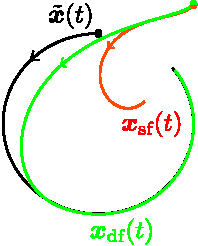
\includegraphics[height=\textwidth]{methods/reference_trajectory}
    \caption{Dynamic convergence}%
    \label{subfig:reference_trajectory_1}
  \end{subfigure}%
  \begin{subfigure}{0.5\linewidth}
    \centering
    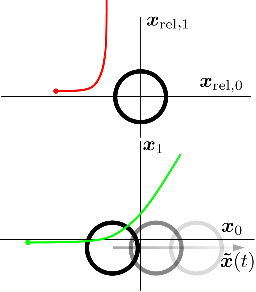
\includegraphics[height=\textwidth]{methods/reference_pull_no_equations}
    \caption{Dynamic Avoidance}%
    \label{subfig:reference_trajectory_2}
  \end{subfigure}
  \caption{The two implications of \acl{df}. 
    In (a), it can be seen that the trajectory obtained with \ac{df} (green)
    converges towards the reference trajectory (black) while the trajectory
    with \acl{sf} (red) does not converge. 
    In (b), the top part
    visualizes collision avoidance as suggested in~\cite{Ratliff2020}. Here,
    the trajectory and obstacle are expressed
    in a relative system $\xr$. Using the dynamic pull, \cref{eq:dynamic_pull}, this
    can be transformed into the static reference frame $\x$, bottom part. Together
    with dynamic energization, the framework of optimization fabrics is leveraged
    for dynamic environments.
    The motion of the obstacle, $\xr(t)$ is visualized with an arrow, future positions
    of the obstacle are shown in lighter color. The resulting trajectory obtained with
    \ac{df} is shown in green.
  }%
  \label{fig:reference_trajectory}
\end{figure}

\subsection{Dynamic pullback}%
\label{sub:dynamic_pullback}

%Specs can be formulated with the relative coordinate \xr{}, as described in
%\cite{Ratliff2020}. 
%The theory remains valid with relative coordinates when all components
%are defined in the same relative coordinates.
The theory of optimization fabrics also applies to relative coordinates \xr{}, specifically,
specs and potentials can be formulated in moving coordinates. However, 
there is no theory to combine specs defined in relative coordinates with specs in fixed
coordinates.
In most cases, individual components of the
behavior design are not formulated in the same relative coordinates. Specificially, the
configuration space is always static, so we introduce a transformation of a relative spec
into the static space \X{}. We call this operation \textit{dynamic pullback}.
\begin{equation}
  \pull{\mapd}{{(\Md,\fd)}_{\Xr}} = {(\Md, \fd - \Md\xtddot)}_{\X}
  \label{eq:dynamic_pull}
\end{equation}
Two specs $\Spec_{\X_{\textrm{rel,1}}}$ and $\Spec_{\X_{\textrm{rel,2}}}$ defined
in two different relative coordinate systems are then combined by
first applying the dynamic pullback to both individually and then applying the summation
operation for specs. The dynamic pullback is the natural extension to optimization fabrics
for relative coordinate systems. It cannot directly be
integrated into the framework of optimization
fabrics as it breaks the algebra. In the following, we derive several
generalizations so that the theory remains 
valid even in the presence of reference trajectories for individual components, such as moving
obstacles or reference trajectories.

\subsection{Dynamic Lagrangians}%
\label{sub:dynamic_lagrangians}

Next, we show that energy conservation commutes with the dynamic pullback. This allows us to
transfer findings on conservative fabrics to dynamic fabrics.
We call a Lagrangian that is defined using relative coordinates
a \textit{dynamic Lagrangian} and write $\ld(\xr, \xrdot)$. 
In this relative coordinate system, the dynamic
Lagrangian has the same properties as the Lagrangian defined in~\cite{Ratliff2020},
specifically it induces the Lagrangian spec through the Euler-Lagrange equation, 
$\dertwo{\xrdot\xrdot}{\ld}\xrddot + \dertwo{\xrdot\xr}{\ld}\xrdot - \der{\xr}{\ld}$, 
as $(\Mde,\fde)$. The system's Hamiltonian $\hd = \der{\xrdot}{\ld}^T\xrdot - \ld$ is
conserved by the equation of motion as proven in~\cite{Ratliff2020}.

Applying the dynamic pullback to the dynamic Lagrangian we obtain the transformed
Lagrangian $\ld(\x, \xdot, \xt, \xdot)$ in the static coordinate system.

\begin{theorem}
  Let $\ld(\xr,\xrdot)$ be a dynamic Lagrangian and let \mapd{} be
  the dynamic mapping to \xr{}. Then, the application of the Euler-Lagrange equation
  commutes with the dynamic pullback.
  \label{the:dynamic_euler_lagrange}
\end{theorem}

\begin{proof}
  We will show the equivalence by calculation. As shown above, the induced spec is defined
in the relative system as $(\Mde, \fde)$. It can be dynamically pulled to form
\begin{equation}
  \pull{\mapd}{{(\Mde,\fde)}_{\Xr}} = {(\Mde, \fde - \Mde\xtddot)}_{\X}
  \label{eq:proof_theorem_euler_commutes}
\end{equation}
We can dynamically pull the Lagrangian $\ld(\xr,\xrdot)$
to form $\ld(\x,\xdot,\xt,\xtdot)$, where only the first two variables are system
variables. Using the generalized Euler-Lagrange equation, the equations of motion of the
pulled Lagrangian are obtained as
\begin{align*}
  0 &= \dert{\derf{\xdot}{\ld}}
      - \derf{\x}{\ld} \\
    &=  \derftwo{\xdot}{\xdot}{\ld}\xddot
      + \derftwo{\xdot}{\x}{\ld}\xdot
      + \derftwo{\xdot}{\xtdot}{\ld}\xtddot
      + \derftwo{\xdot}{\xt}{\ld}\xtdot
      - \derf{\x}{\ld} \\
    &=  \derftwo{\xrdot}{\xrdot}{\ld}\derf{\xdot}{\xrdot}\derf{\xdot}{\xrdot}\xddot 
      + \derftwo{\xrdot}{\xr}{\ld}\derf{\xdot}{\xrdot}\derf{\x}{\xr}\xdot \\
      &+ \derftwo{\xrdot}{\xrdot}{\ld}\derf{\xdot}{\xrdot}\derf{\xtdot}{\xrdot}\xtddot
      + \derftwo{\xrdot}{\xr}{\ld}\derf{\xdot}{\xrdot}\derf{\xt}{\xr}\xtdot \\
      &- \derf{\xr}{\ld}\derf{\x}{\xr} \\
    &=  \derftwo{\xrdot}{\xrdot}{\ld}\xddot
      + \derftwo{\xrdot}{\xr}{\ld}\xdot
      - \derftwo{\xrdot}{\xrdot}{\ld}\xtddot \\
      &- \derftwo{\xrdot}{\xr}{\ld}\xtdot
      - \derf{\xr}{\ld} \\
    &=  \derftwo{\xrdot}{\xrdot}{\ld}(\xddot - \xtddot)
      + \derftwo{\xrdot}{\xr}{\ld}(\xdot - \xtdot)
      - \derf{\xr}{\ld} \\
    &=  \derftwo{\xrdot}{\xrdot}{\ld}(\xddot - \xtddot)
      + \derftwo{\xrdot}{\xr}{\ld}(\xrdot)
      - \der{\xr}{\ld} \\
    &= \Mde \xddot + \fde - \Mde\xtddot
\end{align*}
The obtained equations of motion match the one obtained by applying the dynamic pullback,
see \cref{eq:proof_theorem_euler_commutes}.
\end{proof}
Hence, independently of the coordinates, the system conserves the energy \hd{} computed with the
Hamiltonion in relative coordinates.
Next, we adapt the operation of energization to dynamic Lagrangians. 
Dynamic Lagrangians are a necessary step to allow
for collision avoidance with dynamic obstacles in the framework of
optimization fabrics.
Specifically, the metric for a moving obstacle is computed
using the Euler-Lagrange equation in the relative coordinate system. Importantly, 
in this system, the same energies as with \ac{sf} can be employed. Using the dynamic
pullback, the energy defining the metric for the moving obstacle is then maintained
according to \cref{the:dynamic_euler_lagrange}. Concretely, this means that
collision avoidance can be achieved in a similar manner as with \ac{sf} with the added
advantage of integrated motion estimates of obstacles.

\begin{proposition}[Dynamic Energization]
  Let ${\xddot + \vec{h}(\x,\xdot) = \vec{0}}$ be a differential equation and suppose \ld{} is a
dynamic Lagrangian with the induced spec $(\Mde,\fde)$ and dynamic energy \hd{}. Then the
dynamically energized system~{$\xddot + \vec{h}(\x,\xdot) + \alpha_{\hd}\xrdot = \vec{0}$} with 
\[
  \alpha_{\hd} = -{(\xrdot^T\Mde\xrdot)}^{-1}\xrdot^T(\Mde(\vec{h}+\xtddot)-\fde)
\]
conserves the dynamic energy \hd{}.%
\label{prop:dynamic_energization}
\end{proposition}
\begin{proof}
  From the derivations in~\cite{Ratliff2020}, we can compute the rate of change of the
dynamic energy as $\dot{\hd} = \xrdot^T(\Mde\xrddot + \fde)$. The equations of motion can be
plugged in through the definition of the reference trajectory \cref{def:refTraj}, 
$\xrddot = \xddot - \xtddot$ to obtain:
\begin{align*}
  \dot{\hd} &= \xrdot^T(\Mde(-\vec{h}-\alpha_{\hd}\xrdot - \xtddot) + \fde) \\
  &= \xrdot^T(-\Mde\vec{h}-\Mde\xrdot\alpha_{\hd} - \Mde\xtddot + \fde) \\
  &= \xrdot^T(-\Mde\vec{h} \\
      & +\Mde\xrdot{(\xrdot^T\Mde\xrdot)}^{-1}\xrdot^T(\Mde(\vec{h}+\xtddot)-\fde) \\
      & - \Mde\xtddot + \fde) \\
  &= -\xrdot^T\Mde\vec{h}
      +\xrdot^T(\Mde(\vec{h}+\xtddot)-\fde) \\
      & - \xrdot^T\Mde\xtddot + \xrdot^T\fde \\
  &= 0
\end{align*}
The energized system conserves the dynamic energy.
\end{proof}
\cref{prop:dynamic_energization} allows to combine dynamic components of the
motion generator
with static components. Effectively, the dynamic component \textit{bends} the
underlying geometry according to the motion of the dynamic components (e.g., a moving
obstacle).

While dynamic Lagrangians and the corresponding energization operation are similar to the
methods described in~\cite{Ratliff2020}, the operation of the standard pull to the
dynamically energized system must be slightly modified. Specifically, the reference
velocity must be pulled. We show that dynamic
energization also commutes with the standard pullback.

\begin{theorem}
Let \ld{} be a dynamic Lagrangian to the reference trajectory \xt{}, and
let~{$\xddot+\h(\x, \xdot) = \vec{0}$} be a second order differential equation with a metric \Md{}
such that $\Jt\Md\J$ has full rank that can be written as spec $(\Md, \Md\h)$. Suppose $x =
\map(\q)$ is a differential map with \J{} its Jacobian. Then
\begin{equation}
  \energize{\pull{\map}{\ld}}{\left(\pull{\map}{(\I, \h)}\right)} =
\pull{\map}{\left(\energize{\ld}{(\I,\h)}\right)}, 
\end{equation}
when the reference velocity is being pulled as $\qtdot = \pinv{\J}\xtdot$.
$\pinv{\J}$ denotes the pseudo-inverse of \J{}.
%
We say that the dynamic energization operation commutes with the pullback transform.
\end{theorem}
\begin{proof}
  The commutation can be proven by calculation. First, we compute the right side of the
equivalence. According to \cref{prop:dynamic_energization}, the energized system (that
maintains the dynamic energy \hd{}) writes as 
\[
  \Md\xddot + \Md\h + \alpha_{\hd}(\xdot-\xtdot) = 0, 
\]
with $\alpha_{\hd}$ as defined in \cref{prop:dynamic_energization}.
Applying the pull-operation, we obtain
\begin{equation}
  \Jt\Md\J\qddot + \Jt\Md\h + \Jt\Md\Jdot\qdot + \Jt\Md\alpha_{\hd}(\xdot-\xtdot) = 0.
  \label{eq:pulled_energized_system}
\end{equation}
As the equation expressed in \X{}, this equation in \Q{} maintains the energy \hd{}. Next,
we compute the left hand side. The equation of motion of the pulled dynamic Lagrangian \ld{}
computes as 
\begin{align*}
  \pull{\map}{(\Md,\fd)}
    &= \Jt\left(\Md\J\qddot  + \fd + \Md\Jdot\qdot - \Md\xtddot\right)\\
    &= \tilde{\Md}\qddot  + \tilde{\fd} - \Jt\Md\xtddot.
\end{align*}
The original spec is pulled accordingly
\begin{align*}
  \pull{\map}{(\Md,\Md\h)} &=
  \Jt\Md\J\qddot + \Jt\Md\h + \Jt\Md\Jdot\qdot \\
  &= \tilde{\Md}\qddot + \tilde{\Md}\tilde{\h}
\end{align*}
We energize the pulled system according to \cref{prop:dynamic_energization}
\begin{equation}
  \begin{split}
    \Jt\Md\J\qddot + \Jt\Md\h + \Jt\Md\Jdot\qdot \\
    + \Jt\Md\J\alpha_{\pull{\map}{\hd}}(\qdot-\pinv{\J}\xdot) = 0, 
  \end{split}
\label{eq:energized_pulled_system}
\end{equation}
with 
\begin{align*}
  \alpha_{\pull{\map}{\hd}} = 
    & -{\left({(\qdot-\pinv{\J}\xtdot)}^T\Jt\Md\J(\qdot-\pinv{\J}\xtdot)\right)}^{-1} \\
    & {(\qdot-\pinv{\J}\xtdot)}^T\left(\Jt\Md\J(\tilde{\h}+\xtddot)\right. \\
    & - \left.\Jt\fd - \Jt\Md\Jdot\qdot\right) \\
    = & -{\left({(\J\qdot-\J\pinv{\J}\xtdot)}^T\Md(\J\qdot-\J\pinv{\J}\xtdot)\right)}^{-1} \\
    & {(\qdot-\pinv{\J}\xtdot)}^T\left(\Jt\Md\J\tilde{\h}+\Jt\Md\xtddot\right. \\
    & \left.- \Jt\fd - \Jt\Md\Jdot\qdot\right) \\
    = & -{\left({(\xdot-\xtdot)}^T\Md(\xdot-\xtdot)\right)}^{-1} \\
    & {(\qdot-\pinv{\J}\xtdot)}^T\left(\Jt\Md\h + \Jt\Md\Jdot\qdot +\Jt\Md\xtddot\right. \\
    & \left.- \Jt\fd - \Jt\Md\Jdot\qdot\right) \\
    = & -{\left({(\xdot-\xtdot)}^T\Md(\xdot-\xtdot)\right)}^{-1} \\
    & {(\qdot-\pinv{\J}\xtdot)}^T\left(\Jt\Md\h + \Jt\Md\xtddot- \Jt\fd \right) \\
    = & -{\left({(\xdot-\xtdot)}^T\Md(\xdot-\xtdot)\right)}^{-1} \\
    & {(\J\qdot-\J\pinv{\J}\xtdot)}^T\left(\Md\h + \Md\xtddot- \fd \right) \\
    = & -{\left({(\xdot-\xtdot)}^T\Md(\xdot-\xtdot)\right)}^{-1}
    {(\xdot-\xtdot)}^T\\
    & \left(\Md\h + \Md\xtddot- \fd \right) \\
    & = \alpha_{\hd}
\end{align*}
Thus, we have shown equivalence between $\alpha_{\hd}$
and $\alpha_{\pull{\map}{\hd}}$. As $\alpha$ is scalar we can can rewrite the energization
term in \cref{eq:energized_pulled_system} as
\begin{align*}
  &\Jt\Md\J\alpha_{\pull{\map}{\hd}}(\qdot-\pinv{\J}\xdot)\\
  = &\Jt\Md\alpha_{\pull{\map}{\hd}}(\J\qdot-\J\pinv{\J}\xdot)\\
  = &\Jt\Md\alpha_{\pull{\map}{\hd}}(\xdot-\xdot)\\
  = &\Jt\Md\alpha_{\hd}(\xdot-\xdot)\\
\end{align*}
With the equivalence of the energization terms, we conclude the
proof that dynamic energization commutes with the standard pullback.
\end{proof}

\subsection{Dynamic fabrics}%
\label{sub:dynamic_fabrics}

With the previous results, we formulate a new class of fabrics that converge to a
reference trajectory. We call this class of fabrics \acl{df}. 
First, some notations are introduced to eventually show that dynamically energized specs
form dynamic fabrics.
%
\iffalse%
\begin{definition}
A spec is called \textit{dynamically converging} towards a reference $\xt(t)$,
if and only if
\[
  \exists t_1 \geq 0, \forall t \geq t_1:
      \xddot(t) = \xtddot(t), \xdot(t) = \xtdot(t), \x(t) = \xt(t),
\]
For clarity, we say that the spec is dynamically converging with respect to $\xt$, or
dynamically converging for short if the reference is clear from the context.
\end{definition}
\fi
%
Analogously to unbiased specs, we define dynamically unbiased specs (i.e., specs whose
solutions do not diverge from the reference \xt{} when starting on the reference).
\begin{definition}
A spec is said to be \textit{dynamically unbiased} with respect to $\xt(t)$ if
$\f(\x, \xdot) = -\M\xtddot$, for $\x(t) = \xt(t)$ and $\xdot(t) = \xtdot(t)$.
\end{definition}

Beside being dynamically unbiased, some specs will converge to the reference trajectory
independently from their initial conditions.

\begin{definition}
A spec is \textit{dynamically rough} with respect to $\xt(t)$ if all
its integral curves $\x(t)$ converge dynamically with respect to $\xt(t)$.
\end{definition}

As for \ac{sf}, \ac{df} can be formed by
specs when they are being forced by a potential function \forc. Such a forcing potential is
generally a function of \x{} and \xt{} and has at least one minimum. A spec that converges
to a minimum of the forcing potential then forms a dynamic fabrics.

\begin{definition}
A spec forms a \textit{dynamically rough fabric} if it is dynamically rough with respect
to $\xt(t)$ when forced by a dynamic potential and 
$\exists t_1 > 0$ such that $\forall t>t_1, \x(t)$ satisfies the
Karush-Kuhn-Tucker (KKT) conditions for the optimization problem $\text{min}_{\x\in\X} \forc(\x,
\xt(t))$. If a spec does not form a dynamically rough fabric but all its damped variants
do, it forms a \textit{dynamically frictionless fabric}.
\end{definition}

\begin{theorem}[Dynamic Fabrics]
%Suppose $S=(\M,\f)_{\X}$ is a dynamic spec with respect to \xt{}.
Suppose $S={(\M,\f)}_{\X}$ is a spec.  Then $S$ forms a dynamically rough fabric with
respect to \xt{} if and only if it is dynamically unbiased with respect to \xt{} and it
converges dynamically when being forced by a dynamic potential $\forc(\x,\xt)$ with
$\norm{\der{\x}{\forc}} < \infty$ on \X{}.%
\label{the:dynamic_fabrics}
\end{theorem}

\begin{proof}
We can write the corresponding differential equation
\begin{equation}
  \M\xddot + \f = -\der{\x}{\forc}
  \label{eq:proof_4_10_b}
\end{equation}
Assume that $S$ is dynamically unbiased.
Since the spec converges with respect to $\xt(t)$, we have $\xdot\to\xtdot, \x\to\xt$.
Because it is dynamically unbiased we also have $\f\to-\M\xtddot$.
Thus, the left hand side of
\cref{eq:proof_4_10_b}, approaches $\vec{0}$.
Consequently, the right hand side must also
approach $\vec{0}$ and hence $\der{\x}{\forc} \to \vec{0}$. The last satisfies the 
Karush–Kuhn–Tucker (KKT)
conditions of \forc{}.

To prove the converse, assume \f{} dynamically biased. That implies that 
\[
  \exists t > 0, \f = \M\xtddot + \vec{a}(\xt, \xtdot),
    \vec{a}(\xt, \xtdot) \neq \vec{0}.
\]
Hence, there exist a $t > 0$ for which the left hand side does not vanish. As \forc{}
satisifies the KKT conditions at $\x = \xt$, its derivative equals zero at $\x = \xt$ which contradicts
\cref{eq:proof_4_10_b} with $\M\vec{a}(\xt, \xtdot) = \vec{0}$.
\end{proof}

Hence, the spec is required to be unbiased and convergent when forced. While the former
can be verified using straight-forward computation, convergence is difficult to verify in
the general case. 

% \MS{Are we sure that dynamically energized specs are dynamically unbiased?}
\begin{lemma}[Dynamically energized fabrics]
  Suppose $S$ is a dynamically unbiased energized spec. Then $S$
  forms a dynamically frictionless
  fabric if  $\der{\x}{\forc} = -\der{\xt}{\forc}$.%
\label{lem:dynamically_energized_fabrics}
\end{lemma}
\begin{proof}
  The equation of motion for the energized, forced and damped system writes as 
  \begin{equation}
    \xddot + \vec{h} + \alpha_{\hd}\xrdot + \mat{B}\xrdot + \der{\x}{\forc} = 0
  \end{equation}
  The systems energy (dynamic Hamiltonian) is used as a Lyapunov function to show
  convergence. The rate of change is computed as
  \begin{align*}
    \dot{\hd^{\forc}} &= \xrdot^T(
      \Mde(
        -\vec{h}
        - \alpha_{\hd}\xrdot 
        - \mat{B}\xrdot 
        - \der{\x}{\forc}
        - \xtddot) \\
      & + \fde) 
      + \dot{\forc} \\
              &= -\xrdot^T\mat{B}\xrdot
      - \xrdot^T\der{\x}{\forc}
      + \xdot^T\der{\x}{\forc}
      + \xtdot^T\der{\xt}{\forc} \\
              &= -\xrdot^T\mat{B}\xrdot \\
  \end{align*}

  As the system energy is lower bounded with $\hd + \forc \geq 0$ and 
  $\dot{\hd^{\forc}} \leq 0$, when $\mat{B}$ stricly positive definite, we must have
$\dot{\hd^{\forc}} \to 0$. Thus, \xrdot{} goes to zero. We can conclude that the system is
dynamically converging. As it it also said to be dynamically unbiased, the damped
energized system forms a dynamic fabric by \cref{the:dynamic_fabrics}.
\end{proof}

\begin{lemma}[Dynamic Lagrangian fabrics]
An unbiased, dynamic Lagrangian spec forms a dynamically frictionless
fabric if  $\der{\x}{\forc} = -\der{\xt}{\forc}$ holds for the forcing term.
\label{lem:dynamic_lagrangian_fabrics}
\end{lemma}
\begin{proof}
The equations of motion induced by the dynamic Lagrangian including damping and forcing 
are defined by the spec and can
be written explicitly as
\begin{align}
  \M_{\ld}\xrddot + \f_{\ld} + \mat{B}\xrdot + \der{\x}{\forc} = 0 \nonumber \\
  \M_{\ld}(\xddot - \xtddot) + \f_{\ld} + \mat{B}(\xdot - \xtdot) + \der{\x}{\forc} = 0
\label{eq:motion} \\
  \M_{\ld}\xddot - \M_{\ld}\xtddot + \f_{\ld} + \mat{B}\xdot - \mat{B}\xtdot +
    \der{\x}{\forc} = 0 \nonumber
\end{align}

In the following we use the Hamiltonian and the potential function as Lyapunov function to
show convergence of the damped spec.
\begin{align*}
  \hd^{\forc}(\x) &= \hd + \forc \\
  &= \der{\xrdot}{\ld^T}\xrdot - \ld + \forc
\end{align*}
The time derivative is composed of the time derivative of the Hamiltonian, $\dot{\he} =
\xrdot^T (\M_{\ld}\xrddot + \f_{\ld})$, and the time derivative of the forcing potential, 
$\dot{\forc} = \xdot^T\der{\x}{\forc} + \xtdot^T\der{\xt}{\forc}$.
Thus, the system's total energy varies over time:
\[
  \dot{\hd}^{\forc}(\x) = {(\xdot - \xtdot)}^T(\M_{\ld} (\xddot - \xtddot) + \f_{\ld}) +
\xdot^T\der{\x}{\forc} + \xtdot^T\der{\xt}{\forc}
\]
Plugging in the equations of motion \cref{eq:motion} gives
\begin{align*}
  \dot{\hd}^{\forc}(\x) &= {(\xdot - \xtdot)}^T(-\f_{\ld} - \mat{B}(\xdot - \xtdot) - \der{\x}{\forc} +
    \f_{\ld}) \\
  &  + \xdot^T\der{\x}{\forc} + \xtdot^T\der{\xt}{\forc} \\
  &= -{(\xdot - \xtdot)}^T\mat{B}(\xdot - \xtdot) - {(\xdot - \xtdot)}^T\der{\x}{\forc} \\
  & + \xdot^T\der{\x}{\forc} + \xtdot^T\der{\xt}{\forc} \\
  &= -{(\xdot - \xtdot)}^T\mat{B}(\xdot - \xtdot)
    + \xtdot^T(\der{\x}{\forc} + \der{\xt}{\forc}).
\end{align*}
For $\der{\x}{\forc} = -\der{\xt}{\forc}$ and $\mat{B}$ strictly positive definite,
$\dot{\hd}$ is strictly negative for $(\xdot - \xtdot) \neq 0$. Since $\hd^{\forc}$ is lower
bounded as composition of lower bounded function and $\dot{\hd}^{\forc} \leq 0$,
$\dot{\hd}^{\forc} \to 0$ and thus, $\xdot \to \xtdot$ and $\x \to \xt$. Hence, the spec
converges dynamically with respect to \xt{}.
As the spec is further said to be
dynamically unbiased, the damped spec forms a dynamic fabric by \cref{the:dynamic_fabrics}.
\end{proof}

Concretely, \cref{lem:dynamic_lagrangian_fabrics} allows for trajectory following
with guaranteed convergence with \ac{df}. For example, a reference trajectory 
for the robot's end-effector is defined as $\xt(t)$. Then, the potential can be designed
as $\psi = \xt(t) - \x$ (respecting the construction rule required
for \cref{lem:dynamic_lagrangian_fabrics}). In contrast to \ac{sf}, where the static
potential function is simply updated at every time step, \ac{df} makes use of the dynamics 
of the reference trajectory through the dynamic pullback.

\subsection{Construction procedure}

From the high-level procedure explained in \cref{sub:motion_design_using_dynamic_fabrics}, we can
derive the algorithm using the formal findings in this section, see \cref{alg:motion_design}.
\begin{algorithm}
  Define basic inertia as spec $\M\qddot + \M\h = 0$ \\
  \For{avoidance in avoidances}{
    Define differential map between \Q{} and $\X_i$: $\map$ or $\map_t$ \\
    Design geometry on $\X_i$: $\xddot_i + \h_{2,i} = \zerovec$ \\
    Design Finsler energy for behavior on $\X_i$: $\l_i$ \\
    Energize geometry with Finsler energy \ref{prop:dynamic_energization}\\
    \If{\map{} is time-parameterized}{
      Apply dynamic pullback to energized system\\
    }
    Apply standard pullback\\
    Add pulled avoidance component to root fabric\\
  }
  Force root system with (time-parameterized) potential\\
  \caption{Motion design with dynamic fabrics}
  \label{alg:motion_design}
\end{algorithm}

Methods to design the individual components, such as geometry and 
Finsler structures, are introduced in~\cite{Ratliff2020}.
As these design patterns do not vary for \ac{df}, they are not repeated here.
In the result section, we show some experimental examples highlighting
the comparative advantage of
optimization fabrics over model predictive schemes and the advantage of \ac{df}
over \ac{sf} for dynamic environments.

